% kuleuventheme2poster by Janez Kren, June 2018, janez.kren@kuleuven.be

\documentclass{beamer}
\usepackage[orientation=portrait,size=a3,scale=1.4,debug]{beamerposter}
% BEAMERPOSTER OPTIONS:
%	orientation= portrait / landscape
%	size= a0 / a2 / a3 / a4
%	scale = change the size of text (e.g. 1.4 increases all fonts by factor of 1.4)


\usetheme[kul,white]{kuleuven2poster}
% THEME OPTIONS 
%	for logo:   kul (default) / kulak / lrd
%	background colour:   blue (default) / white
%	background sedes logo:   no (default) / sedes
%  e.g. [lrd,white,sedes]


% USE YOUR BACKGROUND IMAGE (optinal):
%\titlegraphic{ \includegraphics[height=0.9\paperheight]{mybackground.jpg} } %or, depending on the size: [width=\paperwidth]
%\def\backgdopacity{0.25}  % background image opacity fraction (0=transparent, 1=full colour)

\usepackage{wrapfig}
\usepackage[utf8]{inputenc}
\usepackage{ragged2e}  % enables \justifying


% INFO 
\title{H.A.L.D.I.S.} %Handy Autonomous Lifeless Drink-fetching Instructable Servant
\author{\large Maxim Aelterman, Jarrit Boons, Paul Leroy, Josse Van Delm, Wout Verschaeren}
\institute{\large KU Leuven Campus De Nayer}
\date{}
 

\begin{document}
\csname beamer@calculateheadfoot\endcsname %recalculate head and foot dimension

\begin{frame}[t,fragile]

%%
%%  TITLE HEADER
%%
\vspace{2.5\baseh} % extra vertical space

\begin{tikzpicture}
\node [text width=\textwidth, align=left, inner sep=0pt, outer sep=0, kul-blue, font=\bfseries\fontsize{0.6\baseh pt}{2}\selectfont] 	
{ \inserttitle } ;
% This will create a title larger than \Huge. Can be replaced with the line below, to make it smaller.
\end{tikzpicture}

%\textcolor{kul-blue}{\bfseries \Huge \inserttitle}



%%
%% BODY
%%
\vspace{.2\baseh}

\begin{columns}[T,totalwidth=\textwidth]
% COLUMN 1
	\begin{column}{.48\textwidth}
	The \textbf{Handy Autonomous Lifeless Drink-fetching Instructable Servant} is, as its name suggests, a drink-fetching robot. 
	If you ever feel thirsty behind your desk, HALDIS has got you covered! You'll never have to get out of your comfortable chair again, unless your mum says dinner's ready.
	\break
	\begin{block}{The Mission}
	The main mission of HALDIS can be divided into a number of sub-missions:
	\break
	\begin{column}{.6\textwidth}
	\begin{enumerate}
	    \item Waiting for instruction
	    \break
	    \item Correctly interpreting the instruction
	    \break
	    \item Accurately routing towards the object
	    \break
	    \item Recognising the wanted object 
	    \break
	    \item Firmly grabbing the chosen object
	    \break
	    \item Finding the way back to the user
	    \break
	    \item Releasing object in front of the user 
	\end{enumerate}
	\end{column}
	\begin{column}{.30\textwidth}
    	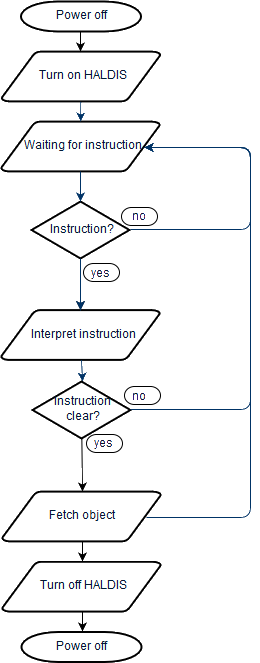
\includegraphics[width=35mm]{graphics/Flowchart.png}
	\end{column}
	\end{block}
	
	\begin{figure}
	    \begin{tabular}{cc}
	        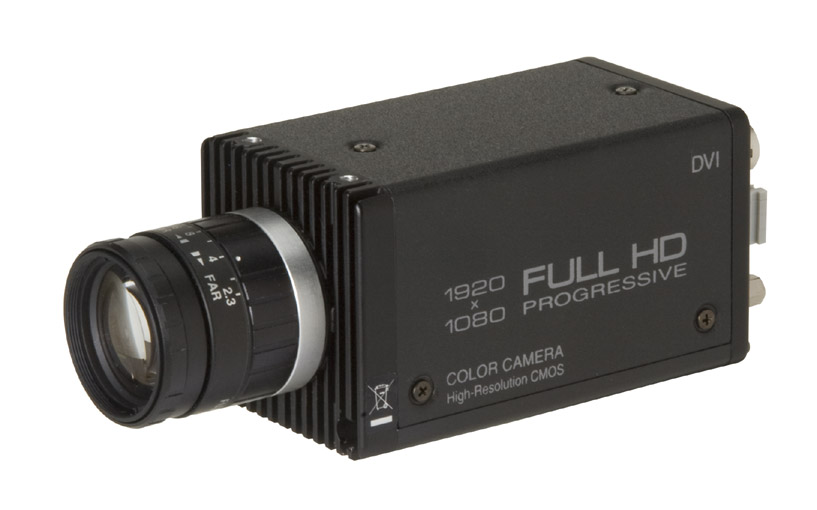
\includegraphics[scale = 0.4]{graphics/camera.jpg}  & 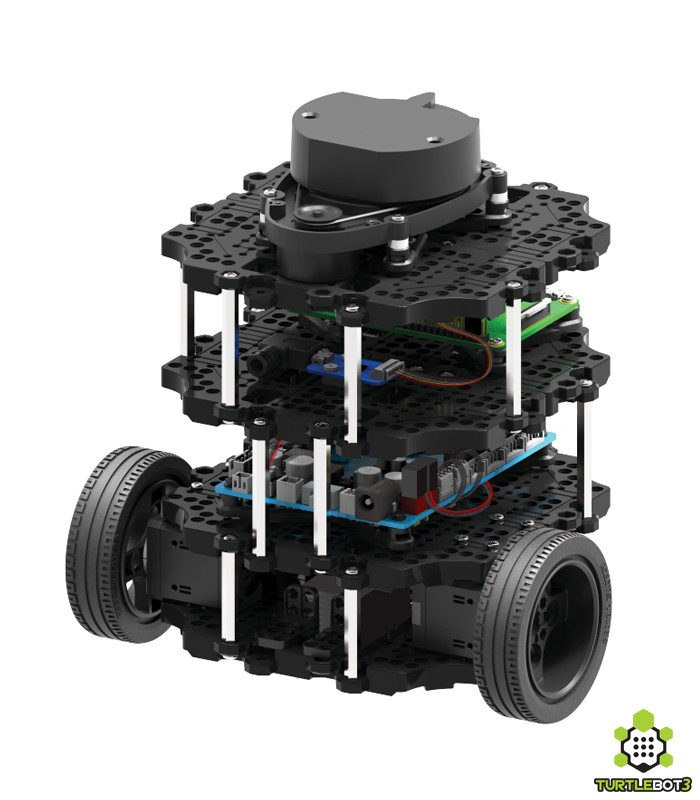
\includegraphics[scale = 0.15]{graphics/turtlebot.jpg} \\
	        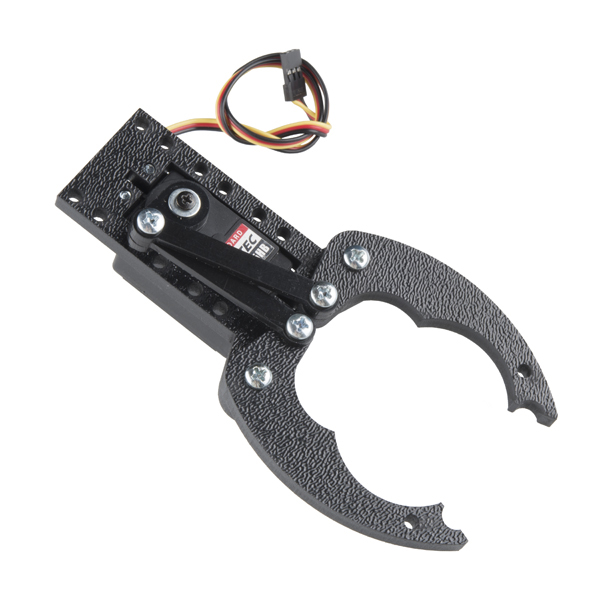
\includegraphics[scale = 0.5]{graphics/claw.jpg}  & 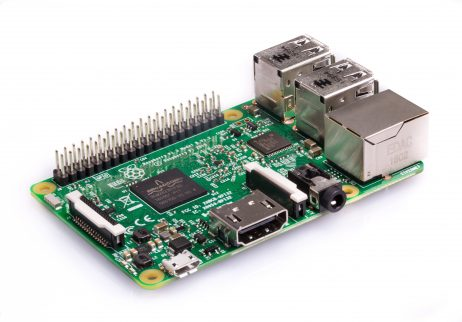
\includegraphics[scale = 0.3]{graphics/rpi.jpg}
	    \end{tabular}
	    \label{fig:fotos}
	    \caption{(LRTB) An RGB camera; The turtlebot 3 burger; A gripper; The raspberry pi 3 model B}
	\end{figure}

	
	
	\end{column}







% COLUMN 2
	\begin{column}{.48\textwidth}
		
	\begin{block}{Robot Concepts Used}
	HALDIS uses a few different robot concepts to fetch your favourite drink. It uses robot vision to scan its surroundings and to move accordingly. 
	When the robot is in place, the vision system identifies the correct object and a gripper is used to grab it.
	All of the robot's actions are guided by the controller. 
	We will discuss these concepts here in more detail (see figure \ref{fig:fotos}).
	
	\begin{exampleblock}{Robot vision (PERCEPTION)}
	For navigation and recognition purposes, we use an \textbf{RGB camera} system with recognition software.
	In a first prototype we use fiducial markers to guide the robot in this process.
	We use \textbf{ArUco} markers for object detection and a \textbf{tape line} on a surface to steer the robot.
	If we have enough time left, we can make a second prototype in which we leave out the markers used to detect the correct object.
	We can then use (deep learning) detection algorithms to detect the correct objects without the use of markers.
	\end{exampleblock}

	\begin{exampleblock}{Robot movement (ACTUATION)}
	When HALDIS is aware of its surroundings it has to move to the target location.
	For this we use the \textbf{motors} and \textbf{wheels} that are included with the robot.
	\end{exampleblock}
	
	\begin{exampleblock}{Gripper (ACTUATION)}
	One of the objectives of our robot is to grab a given object.
	We thus use a \textbf{motorised gripper}, attached to the robot.
	\end{exampleblock}
	
	\begin{exampleblock}{Controller (DECISION)}
	The brains of the robot are the controller. 
	We use the \textbf{raspberry pi} in our setup. 
	If we're able to make the second prototype with detection algorithms, the use of the \textbf{neural compute stick} is also an option. 
	\end{exampleblock}
	
	
	\end{block}
	
	\begin{block}{Planning}
	We visualised our initial planning  using a Gantt chart (see figure \ref{fig:gantt}), by dividing the task into smaller objectives that can be done simultaneously by the different members and implemented in the final system when done. When the main components work properly we can use the spare time to extend some features as described in "Robot Concepts Used".         
	\end{block}
	
	\end{column}


\end{columns}

\begin{figure}
    \centering
    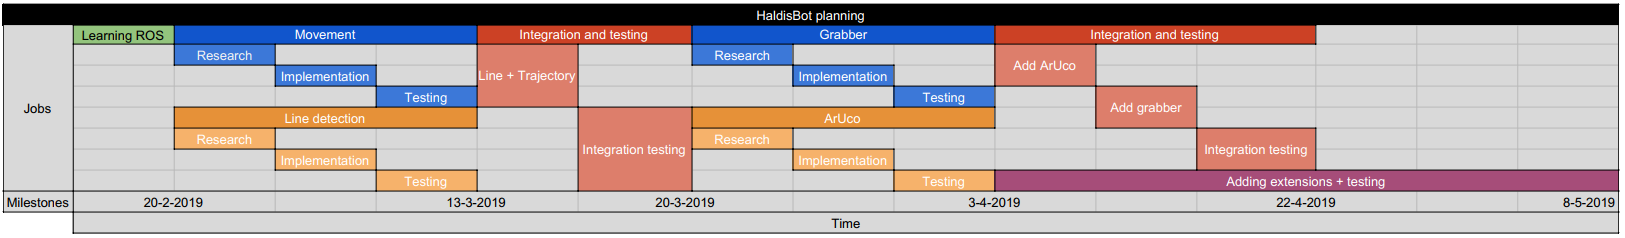
\includegraphics[width=\textwidth]{graphics/planning.png}
    \caption{Gantt chart initial planning}
    \label{fig:gantt}
\end{figure}


\end{frame}

\end{document}